\documentclass{article}

\usepackage{amsmath}
\usepackage{amssymb}
\usepackage{amsthm}
\usepackage{amssymb}
\usepackage{mathdots}
\usepackage[pdftex]{graphicx}
\usepackage{fancyhdr}
\usepackage[margin=1in]{geometry}
\usepackage{multicol}
\usepackage{bbm}
\usepackage{esint}
\usepackage{listings}
\PassOptionsToPackage{usenames,dvipsnames}{color}  %% Allow color names
\usepackage{pdfpages}
\usepackage{algpseudocode}
\usepackage{tikz}
\usepackage[T1]{fontenc}
\usepackage{inconsolata}
\usepackage{framed}
\usepackage{wasysym}
\usepackage[thinlines]{easytable}
\usepackage{wrapfig}
\usepackage{hyperref}
\usepackage{cancel}
\usepackage{tabu}
\usepackage{tabularx}
\usepackage{mathtools}
\usepackage{mathrsfs}
\usepackage{enumerate}
\usepackage{enumitem}
\usepackage{tabto}

\renewcommand{\P}{\mathbb{P}}
\DeclareMathOperator{\N}{\mathbb{N}}
\DeclareMathOperator{\Z}{\mathbb{Z}}
\DeclareMathOperator{\Q}{\mathbb{Q}}
\DeclareMathOperator{\R}{\mathbb{R}}
\DeclareMathOperator{\C}{\mathbb{C}}
\DeclareMathOperator{\F}{\mathbb{F}}
\DeclareMathOperator{\E}{\mathbb{E}}

% Margins
\topmargin=-0.45in
\evensidemargin=0in
\oddsidemargin=0in
\textwidth=6.5in
\textheight=9.0in
\headsep=0.25in

\title{Problem Set 3}
\author{Laker Newhouse\\Collaborators: Evelyn Fu, Jacob Hansen}
\date{\today}

\begin{document}
\maketitle	

All code and raw results are available at \url{https://github.com/Arongil/6.S098/tree/main/pset3}.
\begin{enumerate}
    \item We formulate the problem of finding the maximum likelihood estimate of $x$ given $y$ as a convex optimization problem as follows. We let $x$ be the problem variable. It is $N \times 1$. The objective is that of a least squares problem: we seek to minimize $\| Ax - y \|_2^2$, where $A$ is a matrix we construct for the purpose of converting a raw signal $x$ into the data we would gather: hence the magnitude of $Ax - y$ measures the error of our prediction. The matrix $A$ has the structure \[
        A = \begin{bmatrix}
            h(1) & 0 & 0 & 0 & 0 & \cdots & 0 & 0 \\
            h(2) & h(1) & 0 & 0 & 0 & \cdots & 0 & 0 \\
            h(3) & h(2) & h(1) & 0 & 0 & \cdots & 0 & 0 \\
            \vdots & \vdots & \vdots & \vdots & \vdots & \ddots & \vdots & \vdots \\
            0 & \cdots & h(k) & \cdots & h(1) & \ddots & \vdots & \vdots \\
            \vdots & \vdots & \vdots & \vdots & \vdots & \ddots & \vdots & \vdots \\
            0 & 0 & 0 & 0 & 0 & \cdots & h(2) & h(1)
    \end{bmatrix}.
\] It performs the convolution on $x$ by $h$. Finally, we add a constraint that $Bx \geq 0$, where \[
        B = \begin{bmatrix}
            -1 & 1 & 0 & \cdots & 0 & 0 \\
            0 & -1 & 1 & \cdots & 0 & 0 \\
            0 & 0 & -1 & \cdots & 0 & 0 \\
            0 & 0 & 0 & \cdots & 1 & 0 \\
            0 & 0 & 0 & \cdots & -1 & 1 \\
        \end{bmatrix},
    \] to ensure that $x$ is nondecreasing. We also require $x \geq 0$. Now we consider the specific instance of the problem as given in part (b). The maximum likelihood estimate indeed closely traces the true signal! Interestingly, when we remove the nondecreasing constraint, the estimate becomes erratic -- it is too easy for it to overfit to the noisy data.

    \begin{center}
    	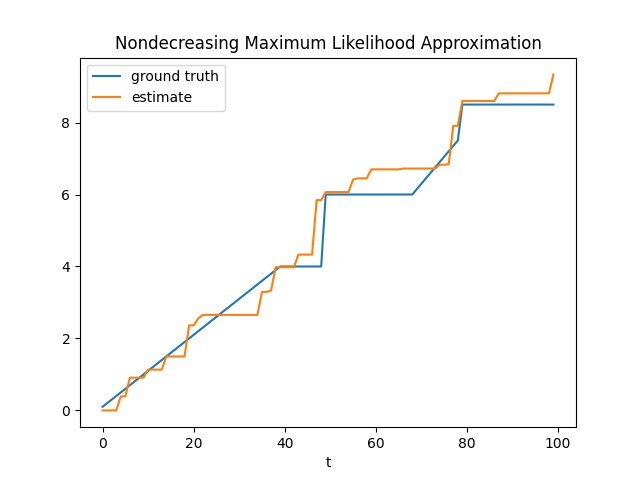
\includegraphics[scale=0.5]{p1_plot_nondecreasing}
    	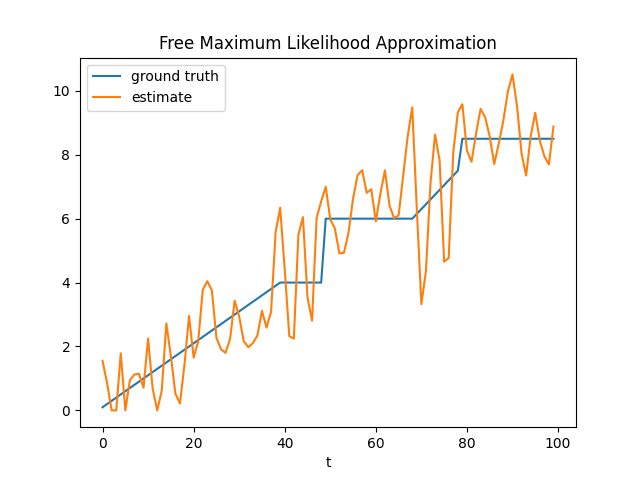
\includegraphics[scale=0.5]{p1_plot_free}
    \end{center}

    \item For the maximum likelihood estimate, we want to maximize the log probability function. We know $p_z(u) = \text{exp}(-\phi(\|u\|_2))$, where $\phi : \R \to \R$ is convex and increasing. The density of $x = Az + b$ is given by the hint to be \[
        p_x(v) = \frac{1}{|\text{det}(A)} p_z(A^{-1}(v - b)).
    \] Therefore, the chance of $x_1, \dots, x_N$ is \[
        \prod \frac{1}{|\text{det}(A)} p_z(A^{-1}(x_i - b)).
    \] The log of this probability becomes a sum: \[
        l(\mathbf{x}) = -N \log(|\text{det}(A)|) - \sum_{i=1}^N \phi(\|A^{-1}x_i - A^{-1} b\|_2).
    \] We switch the problem to minimization and multiply $l$ by $-1$. We introduce new variables $u_i$ to clarify. The problem becomes \begin{align*}
        &\text{minimize } N\log(|\text{det}(A)|) + \sum_{i=1}^N u_i \\
        &\text{subject to } \phi(\|A^{-1} b - A^{-1} x_i \|_2) \leq u_i.
    \end{align*} The issue is that the log determinant function is concave. The solution is to make $Q = A^{-1}$ be the problem variable rather than $A$ itself. Finally then we also set $Z = A^{-1} b$ to ensure we do not multiply variables together in the problem, as this is not DCP. We can solve for $A$ and $b$ from $Q$ and $Z$. Then the problem becomes instead \begin{align*}
        &\text{minimize } -N\log(\text{det}(Q)) + \sum_{i=1}^N u_i \\
        &\text{subject to } \phi(\|Z - Q x_i \|_2) \leq u_i.
    \end{align*} The problem is DCP now! Affine minus affine in the L2 norm is convex. The L2 norm itself is convex, which when passed into $\phi$ remains convex. Therefore the constraints are convex, and the objective is too now that we have flipped the sign of the log determinant.
    
    \item We skip problem 3 for now.

    \item We explain how to find the optimal power vs. utility tradeoff using convex optimization. We want to maximize utility while minimizing power, which is the same as the objective to minimize power minus utility. To account for different preferences in the tradeoff, we define $\lambda \in [0, 1]$ and say \[
            \text{minimize } \lambda \mathbbm{1}^T p - (1 - \lambda) \sum_{j = 1}^n U_j(f_j).
        \] As for constraints, we are given that $Rf \preceq c$ and $p \preceq p^\text{max}$ and $c \geq 0$ and $p \geq 0$. Additionally, we are given that \[
            c_i = \alpha_i \log(1 + \beta_i p_i).
        \] We rearrange this constraint to make it DCP. First, we change $=$ to $\leq$, which leads to an equivalent problems since $c_i$ only serves as an upper bound elsewhere.Second we do some algebra to write \[
            \frac{1}{\beta_i} e^{c_i / \alpha_i} - 1 \leq p_i.
        \] The input to the exponent is convex and increasing, so when plugged into the exponent it remains convex. Then we have convex less than affine ($p_i)$, which is DCP. \\

        Now we implement for the specific case of $m = 20$, $n = 10$, $U_j(x) = \sqrt{x}$ for $j = 1, \dots, n$, $p_i^\text{max} = 10$, $\alpha_i = \beta_i = 1$, and a network topology generated by seeding numpy with $3$ and then asking for $np.round(np.random.random(m, n))$. The plot below shows the optimal power and utility for values of $\lambda$ ranging from $0$ to $1$. On one extreme we see no power at all -- the expense of no utility is forgotten. On the other extreme, we see a massive amount of power given up for a modest boost in utility -- here we forget the expense of power. In the real world, a compromise would yield the most value.

    \begin{center}
    	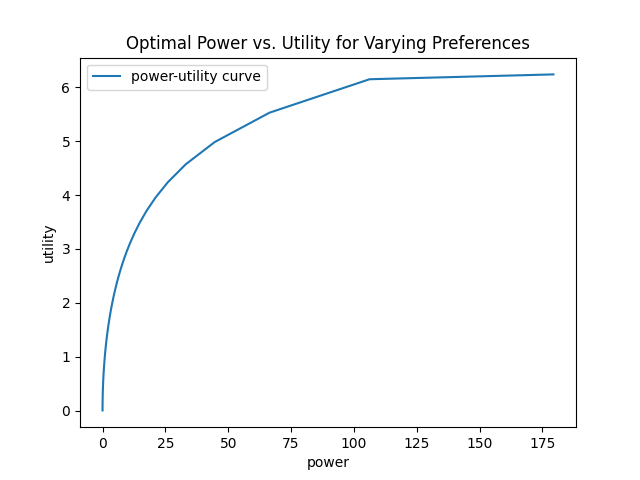
\includegraphics[scale=0.5]{p4_plot}
    \end{center}

    \item I don't believe there is anything I need for the final project at this point. Thank you for your input when I asked last time! I appreciated it and incorporated your advice.
\end{enumerate}
\end{document}
